\documentclass[11pt, A4]{article}
%\usepackage[brazil]{babel}
\usepackage{graphicx}
\usepackage[utf8]{inputenc}
\usepackage[T1]{fontenc}
\usepackage{url}
\usepackage{Sweave}
\usepackage{natbib}
\usepackage{framed, color}
\definecolor{shadecolor}{rgb}{0.9, 0.9, 0.9}
\setlength{\parindent}{0pt}
\setlength{\hoffset}{-0.5in}
\setlength{\textwidth}{6in}
\setlength{\voffset}{-0.1in}
%\pdfpagewidth=\paperwidth
%\pdfpageheight=\paperheight
\newcommand{\R}{{\sf R}}
\newcommand{\code}[1]{\texttt{#1}}



\begin{document}

\title{Fitting species abundance models with maximum likelihood \\ Quick reference for \code{sads} package}
\author{Paulo In\'acio Prado and  Murilo Dantas Miranda \\ Theoretical Ecology Lab \\ LAGE at the Dep of Ecology, USP, Brazil \\ 
  \url{http://ecologia.ib.usp.br/let/} \\ \url{prado@ib.usp.br}}

\date{April, 24, 2014}

\maketitle



\section{Introduction}

Species abundance distributions (SADs) are one of the basic patterns
of ecological communities \citep{McGill2007}. 
The empirical distributions are
traditionally modelled through probability distributions. Hence, the
maximum likelihood method can be used to fit and compare competing
models for SADs. 
The package \code{sads} provides functions to fit the most used models
to empirical SADs and also to evaluate fits and to compare competing
models. The package also allows to simulate SADs expected from samples
from communities, with and without aggregation of individuals of the
same species.


\section{Installation}

The package is planned to be published at CRAN soon. Meanwhile you can install the working version
from GitHub with the package \code{devtools}

\begin{Schunk}
\begin{Sinput}
> library(devtools)
> install_github('sads', 'piklprado')
\end{Sinput}
\end{Schunk}


And then load the package:

\begin{Schunk}
\begin{Sinput}
> library(sads)
\end{Sinput}
\end{Schunk}

\section{Exploratory analyses}
\label{sec:analise-exploratoria}

We'll use two data sets in the sads package:
\begin{Schunk}
\begin{Sinput}
> data(moths)# William's moth data
> data(ARN82.eB.apr77)# Arntz et al. benthos data
\end{Sinput}
\end{Schunk}

\subsection{Octaves}
\label{sec:oitavas}

Function \code{octav} tabulates the number of species in classes
of logarithm of abundances at base 2 (Preston's octaves) and returns a data frame 
\footnote{actually an object of class \emph{octav} which inherits from class \emph{dataframe}}:

\begin{Schunk}
\begin{Sinput}
> (moths.oc <- octav(moths))
\end{Sinput}
\begin{Soutput}
Object of class "octav"
   octave upper Freq
1       1     1   35
2       2     2   11
3       3     4   29
4       4     8   32
5       5    16   26
6       6    32   32
7       7    64   31
8       8   128   13
9       9   256   19
10     10   512    5
11     11  1024    6
12     12  2048    0
13     13  4096    1
\end{Soutput}
\begin{Sinput}
> (arn.oc <- octav(ARN82.eB.apr77))
\end{Sinput}
\begin{Soutput}
Object of class "octav"
   octave      upper Freq
1      -5   0.015625    3
2      -4   0.031250    5
3      -3   0.062500    4
4      -2   0.125000    6
5      -1   0.250000    3
6       0   0.500000    5
7       1   1.000000    2
8       2   2.000000    4
9       3   4.000000    3
10      4   8.000000    1
11      5  16.000000    2
12      6  32.000000    0
13      7  64.000000    1
14      8 128.000000    1
\end{Soutput}
\end{Schunk}

A logical argument
\code{preston} allows to smooth the numbers as proposed by \citet{Preston1948}.

The octave number is the lower limit of the class in log2 scale. 
Hence, for abundance values smaller than one (\emph{e.g.} biomass data) the octave numbers are negative numbers.
A Preston plot is a histogram of this table, that you get applying the function \code{plot} to the data frame:

\setkeys{Gin}{width=0.75\textwidth}
\begin{Schunk}
\begin{Sinput}
> plot(moths.oc)
\end{Sinput}
\end{Schunk}
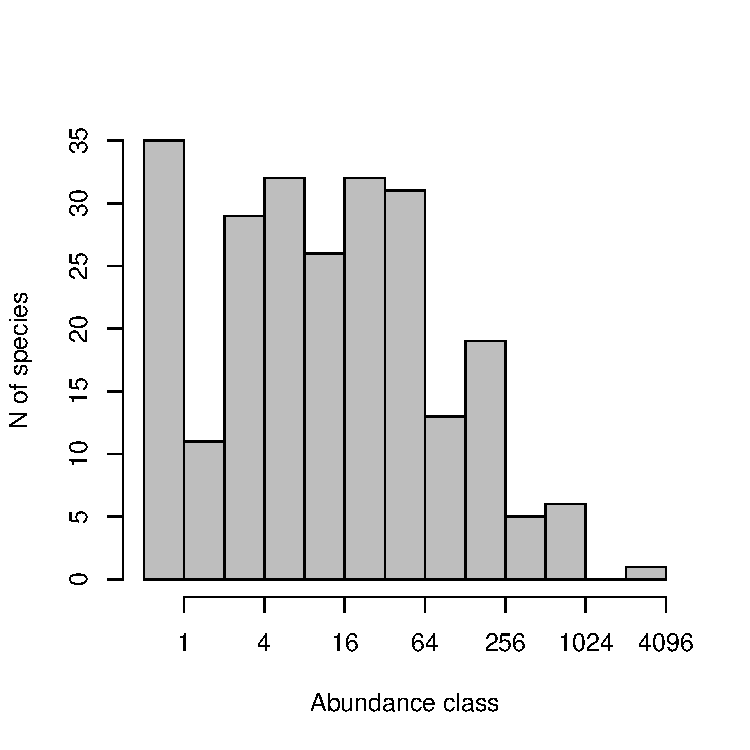
\includegraphics{sads_quick_reference-Ploting-octaves}

\begin{Schunk}
\begin{Sinput}
> plot(arn.oc)
\end{Sinput}
\end{Schunk}
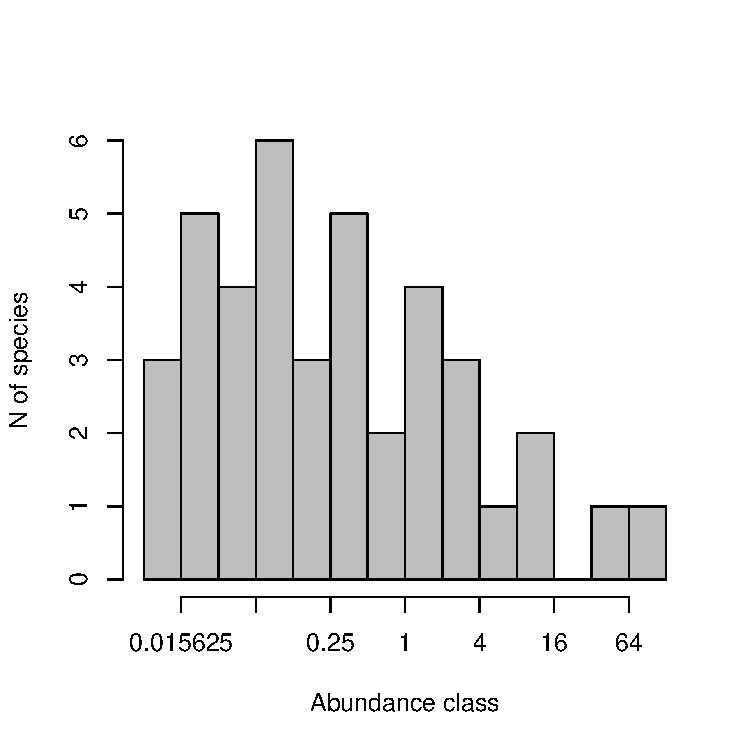
\includegraphics{sads_quick_reference-Biomass-octave-plot}



\subsection{Rank-abundance plots}
\label{sec:rank_abund}
Function \code{rad} returns a data frame of sorted abundances and their ranks 
\footnote{actually an object of class \emph{rad} which inherits from class \emph{dataframe}}:

\begin{Schunk}
\begin{Sinput}
> head(moths.rad <- rad(moths))
\end{Sinput}
\begin{Soutput}
  rank abund
1    1  2349
2    2   823
3    3   743
4    4   604
5    5   589
6    6   572
\end{Soutput}
\begin{Sinput}
> head(arn.rad <- rad(ARN82.eB.apr77))
\end{Sinput}
\begin{Soutput}
     rank abund
sp17    1 67.21
sp11    2 54.67
sp33    3 14.67
sp9     4  9.90
sp30    5  5.71
sp10    6  2.88
\end{Soutput}
\end{Schunk}

To get the rank-abundance or Whitaker's plot apply the function \code{plot} on the data frame:

\setkeys{Gin}{width=0.8\textwidth}

\begin{Schunk}
\begin{Sinput}
> plot(moths.rad, ylab="Number of individuals")
\end{Sinput}
\end{Schunk}
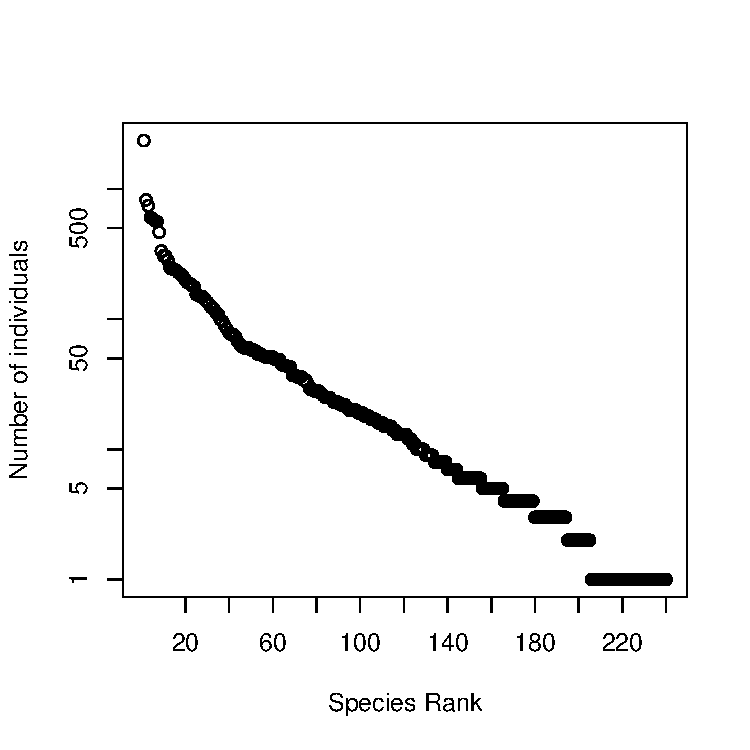
\includegraphics{sads_quick_reference-radplot1}


\begin{Schunk}
\begin{Sinput}
> plot(arn.rad, ylab="Biomass")
\end{Sinput}
\end{Schunk}
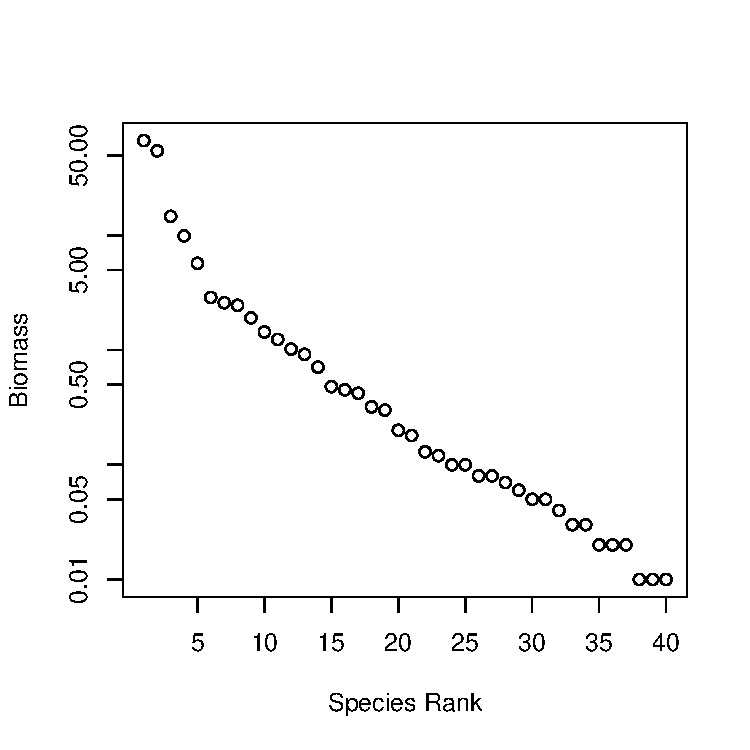
\includegraphics{sads_quick_reference-radplots}

\section{Model fitting}
\label{sec:ajuste-e-selecao}
The \emph{sads} package provides maximum-likelihood fits of many
probability distributions to empirical sads. The working horse is the
functions \code{fitsad} for fitting species abundance distributions
and \code{fitrad} for fitting rank-abundance distributions. The first
argument of these functions is the vector of observed abundances and
the second argument is the name of the model to be fitted.
Please refer to the help
page of the functions for details on the models. For more information
on the fitting procedure see also the vignette of
the \emph{bbmle} package, on top of which the package \emph{sads} is built.

To fit a logseries distribution use the argument \code{sad='ls'}:

\begin{Schunk}
\begin{Sinput}
> (moths.ls <- fitsad(moths,'ls'))
\end{Sinput}
\begin{Soutput}
Call:
mle2(minuslogl = LL, start = list(alpha = alfa), method = "Brent", 
    data = list(x = x), lower = 0, upper = upper)

Coefficients:
   alpha 
40.24728 

Log-likelihood: -1087.71 
\end{Soutput}
\end{Schunk}

The resulting model object inherits from \emph{mle2}
\citep{Bolkerbbmle}, and all usual methods for model objects, such as
summaries, log-likelihood, and AIC values:
\begin{Schunk}
\begin{Sinput}
> summary(moths.ls)
\end{Sinput}
\begin{Soutput}
Maximum likelihood estimation

Call:
mle2(minuslogl = LL, start = list(alpha = alfa), method = "Brent", 
    data = list(x = x), lower = 0, upper = upper)

Coefficients:
      Estimate Std. Error z value     Pr(z)    
alpha   40.247      6.961  5.7818 7.391e-09 ***
---
Signif. codes:  
0 ‘***’ 0.001 ‘**’ 0.01 ‘*’ 0.05 ‘.’ 0.1 ‘ ’ 1

-2 log L: 2175.425 
\end{Soutput}
\begin{Sinput}
> coef(moths.ls)
\end{Sinput}
\begin{Soutput}
   alpha 
40.24728 
\end{Soutput}
\begin{Sinput}
> logLik(moths.ls)
\end{Sinput}
\begin{Soutput}
'log Lik.' -1087.713 (df=1)
\end{Soutput}
\begin{Sinput}
> AIC(moths.ls)
\end{Sinput}
\begin{Soutput}
[1] 2177.425
\end{Soutput}
\end{Schunk}


\subsection{Model diagnostics}
\label{sec:model-diagnostics}
Many other diagnostic and functions are available for sad and rad models. 
To get likelihood profiles and confidence intervals use:

\setkeys{Gin}{width=\textwidth}

\begin{Schunk}
\begin{Sinput}
> moths.ls.prf <- profile(moths.ls)
> confint(moths.ls.prf) # conf intervals
\end{Sinput}
\begin{Soutput}
   2.5 %   97.5 % 
28.01537 55.36267 
\end{Soutput}
\end{Schunk}

And then use \code{plotprofmle} to plot likelihood profiles at the original scale (relative negative log-likelihood)
and function \code{plot} to get plots at chi-square scale (square-root of twice the relative log-likelihood):

\setkeys{Gin}{width=\textwidth}

\begin{Schunk}
\begin{Sinput}
> par(mfrow=c(1,2))
> plotprofmle(moths.ls.prf)# log-likelihood profile
> plot(moths.ls.prf)# z-transformed profile
> par(mfrow=c(1,1))
\end{Sinput}
\end{Schunk}
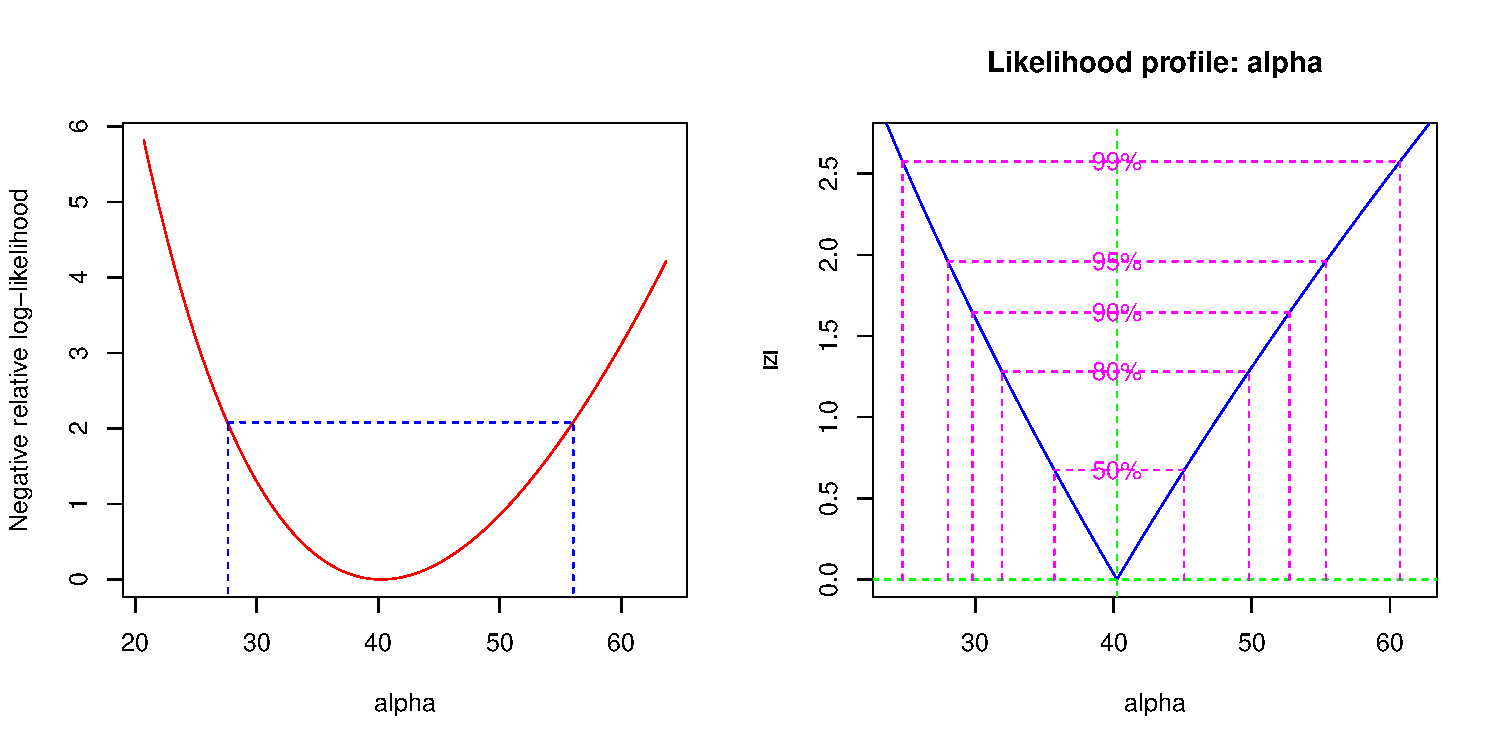
\includegraphics{sads_quick_reference-Ploting-profiles}


When applied on a sad model object the function \code{plot} returns four diagnostic plots:
\begin{Schunk}
\begin{Sinput}
> par(mfrow=c(2,2))
> plot(moths.ls)
> par(mfrow=c(1,1))
\end{Sinput}
\end{Schunk}
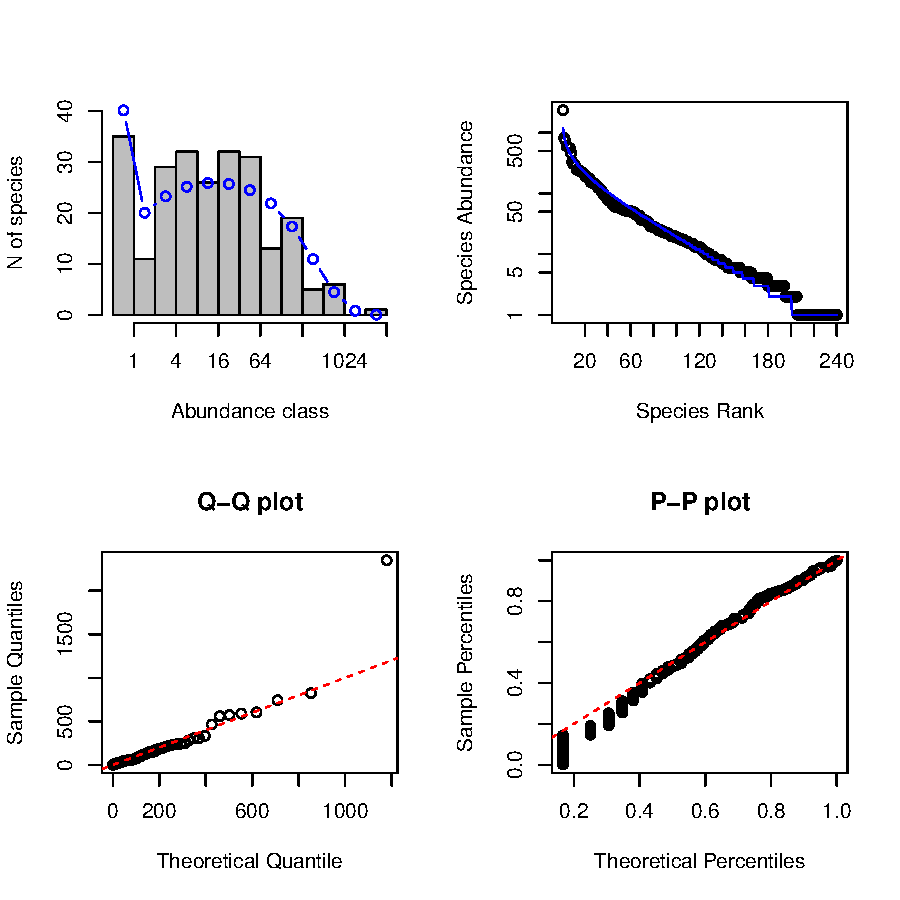
\includegraphics{sads_quick_reference-Plot-of-predicted-values}


The first two plots (top right and left) are the octave and rank-abundance plots with the predicted values 
of number of species in each octave 
and abundances of each species. The two last plots (bottom) are quantile-quantile and percentile-percentile graphs of 
the observed vs. predicted abundances. The straight line indicates the expected relation in case of perfect fit.

\subsection{Rank-abundance models}

Species-abundance models assigns a probability to each abundance
value. Hence these models are probability density functions (PDFs) of
abundances of a species taken at random from the
community. Rank-abundance models assigns a probability for each
\textbf{abundance rank}. They are PDFs for rankings. The models are
interchangeable \citep{May1975}, but currently only four rad models
are available in package sads trough the argument \code{rad} of
function \code{fitrad}:

\begin{itemize}
\item ``gs'': geometric series (which is NOT geometric PDF, available
  in \code{fitsads} as ``geom'';
\item ``rbs'': broken-stick model \citep{macarthur1957, May1975}
\item ``zipf'': zipf power-law distribution
\item ``mand'': zipf-mandelbrot power-law distribution
\end{itemize}

\begin{shaded}
  \textbf{Comparison to \code{radfit} from \emph{vegan} package:} \hfill
  
  fits by \code{fitsad}, \code{fitrad} and \code{radfit} of \emph{vegan} 
  package provide similar estimates of model coefficients 
  but not comparable likelihood values. This is because each function fit models that assigns 
  probability to data in different ways. Function \code{fitsad} fit PDFs to observed abundances and \code{fitrad} fit PDFs 
  to the ranks of the abundances. Finally, \code{radfit} fits a Poisson generalized linear model 
  to the \emph{expected abundances} deduced 
  from rank-abundance relationships from the correspodending sads and rads models \citep{wilson1991}. 
  See also the help page of \code{radfit}. 
  Therefore \textbf{likelihoods obtained from these three functions are not comparable}.
\end{shaded}

\section{Model selection}

You can fit other models to the same data set, such as the Poisson-lognormal and a truncated lognormal:
\begin{Schunk}
\begin{Sinput}
> (moths.pl <- fitsad(x=moths,sad="poilog"))#default is zero-truncated
\end{Sinput}
\begin{Soutput}
Call:
mle2(minuslogl = LL, start = as.list(pl.par), data = list(x = x))

Coefficients:
      mu      sig 
1.996469 2.187126 

Log-likelihood: -1086.07 
\end{Soutput}
\begin{Sinput}
> (moths.ln <- fitsad(x=moths,sad="lnorm", trunc=0.5)) # lognormal truncated at 0.5
\end{Sinput}
\begin{Soutput}
Call:
mle2(minuslogl = LL, start = list(meanlog = meanlog, sdlog = sdlog), 
    data = list(x = x))

Coefficients:
 meanlog    sdlog 
2.274346 2.039740 

Log-likelihood: -1085.47 
\end{Soutput}
\end{Schunk}

and then you can use the function \code{AICtab} and friends from the \emph{bbmle} package to get a model selection table:

\begin{Schunk}
\begin{Sinput}
> AICtab(moths.ls, moths.pl, moths.ln, base=TRUE)
\end{Sinput}
\begin{Soutput}
         AIC    dAIC   df
moths.ln 2174.9    0.0 2 
moths.pl 2176.1    1.2 2 
moths.ls 2177.4    2.5 1 
\end{Soutput}
\end{Schunk}

To compare visually fits first get octave tables:

\begin{Schunk}
\begin{Sinput}
> head(moths.ls.oc <- octavpred(moths.ls))
\end{Sinput}
\begin{Soutput}
  octave upper     Freq
1      1     1 40.14377
2      2     2 20.02026
3      3     4 23.27123
4      4     8 25.12674
5      5    16 25.86285
6      6    32 25.67116
\end{Soutput}
\begin{Sinput}
> head(moths.pl.oc <- octavpred(moths.pl))
\end{Sinput}
\begin{Soutput}
  octave upper     Freq
1      1     1 27.58735
2      2     2 19.48216
3      3     4 26.76472
4      4     8 31.88374
5      5    16 33.16140
6      6    32 30.49061
\end{Soutput}
\begin{Sinput}
> head(moths.ln.oc <- octavpred(moths.ln))
\end{Sinput}
\begin{Soutput}
  octave upper     Freq
1      1     1 15.41886
2      2     2 22.44066
3      3     4 29.13034
4      4     8 33.72746
5      5    16 34.82976
6      6    32 32.08088
\end{Soutput}
\end{Schunk}


and then use \code{lines} to superimpose the predicted values in the octave plot:

\setkeys{Gin}{width=0.75\textwidth}
\begin{Schunk}
\begin{Sinput}
> plot(moths.oc)
> lines(moths.ls.oc, col="blue")
> lines(moths.pl.oc, col="red")
> lines(moths.ln.oc, col="green")
> legend("topright", 
        c("Logseries", "Poisson-lognormal", "Truncated lognormal"), 
        lty=1, col=c("blue","red", "green"))
\end{Sinput}
\end{Schunk}
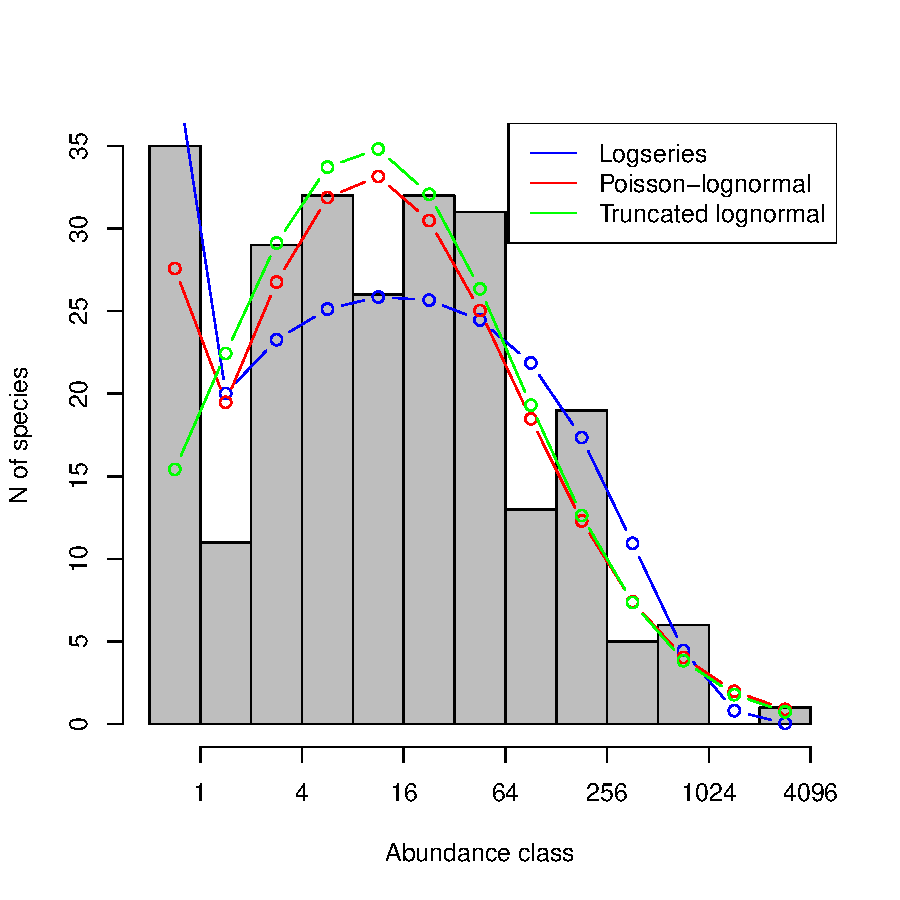
\includegraphics{sads_quick_reference-Octaves-plot}


To do the same with rank-abundance plots get the rank-abundance objects:

\begin{Schunk}
\begin{Sinput}
> head(moths.ls.rad <- radpred(moths.ls)) 
\end{Sinput}
\begin{Soutput}
  rank abund
1    1  1180
2    2   854
3    3   710
4    4   619
5    5   554
6    6   503
\end{Soutput}
\begin{Sinput}
> head(moths.pl.rad <- radpred(moths.pl))
\end{Sinput}
\begin{Soutput}
  rank abund
1    1  4348
2    2  1973
3    3  1322
4    4  1001
5    5   807
6    6   676
\end{Soutput}
\begin{Sinput}
> head(moths.ln.rad <- radpred(moths.ln))
\end{Sinput}
\begin{Soutput}
  rank     abund
1    1 3524.2394
2    2 1674.8603
3    3 1148.3539
4    4  883.6309
5    5  720.7864
6    6  609.2707
\end{Soutput}
\end{Schunk}

and then plot observed and predicted values:

\begin{Schunk}
\begin{Sinput}
> plot(moths.rad)
> lines(moths.ls.rad, col="blue")
> lines(moths.pl.rad, col="red")
> lines(moths.ln.rad, col="green")
> legend("topright", 
        c("Logseries", "Poisson-lognormal", "Truncated lognormal"), 
        lty=1, col=c("blue","red", "green"))
\end{Sinput}
\end{Schunk}
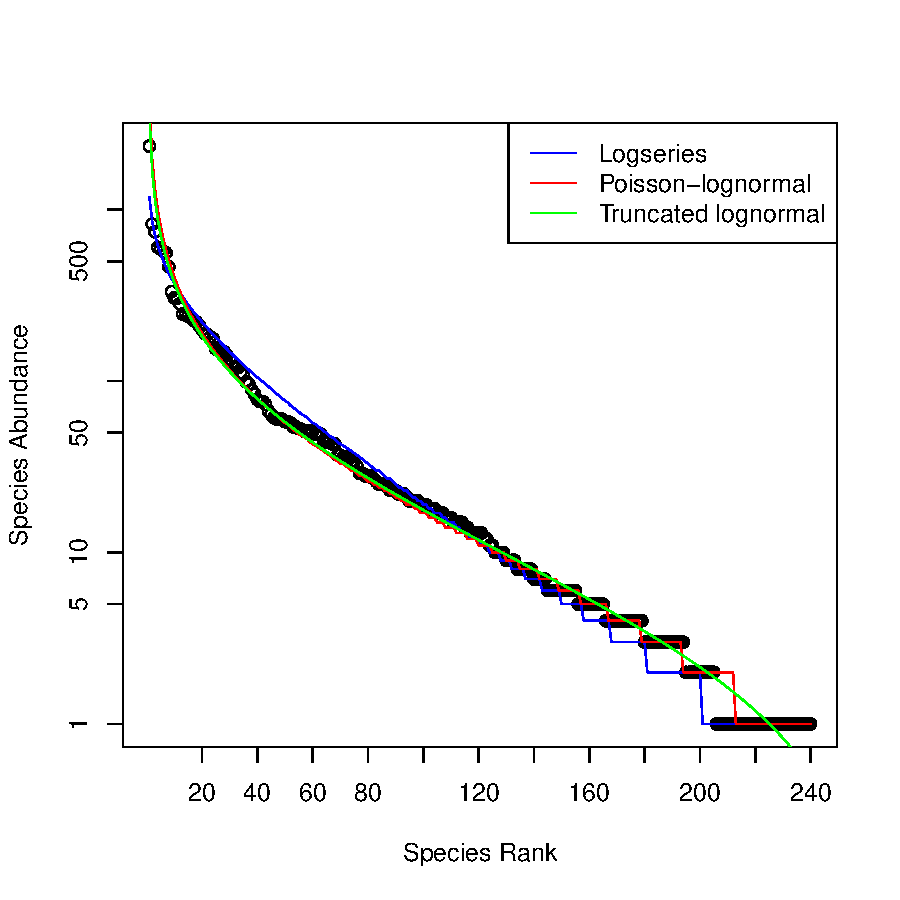
\includegraphics{sads_quick_reference-Rad-plots}

\section{Simulations}

The function \code{rsad} returns random samples of a community which
has $S$ species. The mean abundance of the species in the communities
are independent identically distributed (\emph{iid}) variables that
follow a given probability distribution. The sample simulates a given
number of draws of a fraction $a$ of the total number of individuals of
the community. For instance, to simulate two Poisson samples of 10\%
of a community with 10 species that follows a lognormal distribution
with parameters $\mu=3$ and $\sigma=1.5$ use:

\begin{Schunk}
\begin{Sinput}
> set.seed(42)# fix random seed to make example reproducible
> (samp1 <- rsad(S = 10, frac = 0.1, sad = "lnorm", zeroes=TRUE,
                ssize = 2, meanlog = 3, sdlog = 1.5))
\end{Sinput}
\begin{Soutput}
   sample species abundance
1       1       1        20
2       1       2         4
3       1       3         7
4       1       4         2
5       1       5         4
6       1       6         1
7       1       7        25
8       1       8         3
9       1       9        45
10      1      10         1
11      2       1        17
12      2       2         2
13      2       3         0
14      2       4         3
15      2       5         6
16      2       6         2
17      2       7        18
18      2       8         0
19      2       9        53
20      2      10         4
\end{Soutput}
\end{Schunk}

The function returns a data frame with a sample numeric label,
species numeric label and species abundance in each sample. By
default, \code{rsad} returns a vector of abundances of single Poisson
sample with zeroes ommited:

\begin{Schunk}
\begin{Sinput}
> (samp2 <- rsad(S = 100, frac=0.1, sad="lnorm", 
               meanlog=5, sdlog=2))
\end{Sinput}
\begin{Soutput}
 [1]  155  697    4    7   48    5   40   56  105    8   48
[12]    1    3    1   14   21    6   66    2    3   32  259
[23]    8   51   21    1  312   42   23   20   48   12   28
[34]   14   20   40  267    5  209   36  107   93   58    1
[45]    7   39    2    7   56   70   31    3    4  305   25
[56]   15   12    3   48    8   12  101   69  255    5   51
[67]  253    4    1    2   17   49  187  121  599    3   23
[78]   12    9   16   21   10   17    3    5    2    9    5
[89] 3214    1   19    1   31
\end{Soutput}
\end{Schunk}

Once this is a Poisson sample of a lognormal community, the abundances
in the sample should follow a Poisson-lognormal distribution with
parameters $\mu + \log a $ and $\sigma$
\citep{grotan2008}. We can check this by fitting a Poisson-lognormal
model to the sample:

\begin{Schunk}
\begin{Sinput}
> (samp2.pl <- fitsad(samp2, 'poilog'))
\end{Sinput}
\begin{Soutput}
Call:
mle2(minuslogl = LL, start = as.list(pl.par), data = list(x = x))

Coefficients:
      mu      sig 
2.709138 1.884220 

Log-likelihood: -453.22 
\end{Soutput}
\begin{Sinput}
> ## checking correspondence of parameter mu
> coef(samp2.pl)[1] - log(0.1)
\end{Sinput}
\begin{Soutput}
      mu 
5.011723 
\end{Soutput}
\end{Schunk}

Not bad. By repeating the sampling and the fit many times you can
evaluate the bias and variance of the maximum likelihood estimates:

\setkeys{Gin}{width=\textwidth}
\begin{Schunk}
\begin{Sinput}
> results <- matrix(nrow=500,ncol=2)
> for(i in 1:500){
     x <- rsad(S = 100, frac=0.1, sad="lnorm", 
               meanlog=5, sdlog=2)
     y <- fitsad(x, "poilog")
     results[i,] <- coef(y)
 }
> results[,1] <- results[,1]-log(0.1)
\end{Sinput}
\end{Schunk}

Bias is estimated as the difference between the mean of estimates and
the value of parameters

\begin{Schunk}
\begin{Sinput}
> ##Mean of estimates
> apply(results,2,mean)
\end{Sinput}
\begin{Soutput}
[1] 4.983124 1.993854
\end{Soutput}
\begin{Sinput}
> ## relative bias
> (c(5,2)-apply(results,2,mean))/c(5,2)
\end{Sinput}
\begin{Soutput}
[1] 0.003375221 0.003072756
\end{Soutput}
\end{Schunk}

And the precision of the estimates are their standard deviations

\begin{Schunk}
\begin{Sinput}
> ##Mean of estimates
> apply(results,2,sd)
\end{Sinput}
\begin{Soutput}
[1] 0.2869798 0.2180105
\end{Soutput}
\begin{Sinput}
> ## relative precision
> apply(results,2,sd)/apply(results,2,mean)
\end{Sinput}
\begin{Soutput}
[1] 0.05759033 0.10934122
\end{Soutput}
\end{Schunk}

Finally, a density plot with lines indicating the mean of estimates and the values of parameters:
\begin{Schunk}
\begin{Sinput}
> par(mfrow=c(1,2))
> plot(density(results[,1]-log(0.1)))
> abline(v=c(mean(results[,1]-log(0.1)),5), col=2:3)
> plot(density(results[,2]))
> abline(v=c(mean(results[,2]), 2), col=2:3)
> par(mfrow=c(1,1))
\end{Sinput}
\end{Schunk}
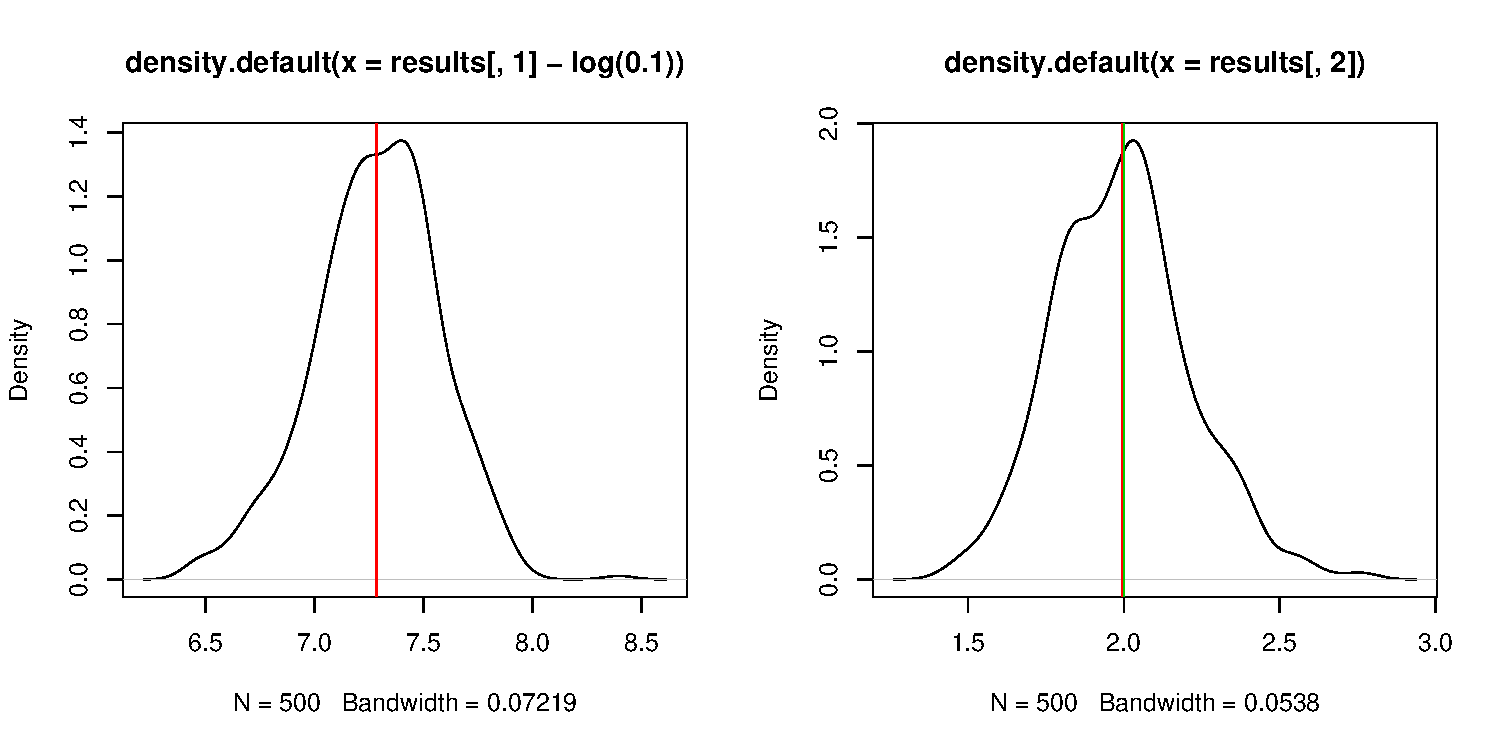
\includegraphics{sads_quick_reference-rsads-bias-plots}


\bibliographystyle{ecology}
\bibliography{sads_quick_reference}
\end{document}
